\documentclass[conference]{IEEEtran}
\IEEEoverridecommandlockouts

\usepackage{cite}
\usepackage{amsmath,amssymb}
\usepackage{graphicx}
\usepackage{booktabs}
\usepackage{url}
\usepackage[hidelinks,pdfauthor={},pdftitle={},pdfsubject={},pdfkeywords={},pdfcreator={}]{hyperref}

\begin{document}

\title{Attackers Learn Twice: Survivorship Bias Hides\\ Within-Attacker Learning in Adaptive Red-Teaming}

\author{\IEEEauthorblockN{Anonymous Author(s)}
\IEEEauthorblockA{\textit{Paper under double-blind review}\\
\textit{Submitted to IEEE SaTML}}
}

\maketitle

\begin{abstract}
How quickly do adversaries learn to defeat a defense? The standard answer comes from the aggregate learning curve: attack success rate as a function of attempt index, pooled across attackers. Across the two largest public corpora of real adaptive human attacks on LLM defenses, LLMail-Inject (461,613 submissions) and Tensor Trust (414,734), that curve falls monotonically: by 60$\times$ in Tensor Trust, and in 48 of 48 LLMail defense cells. Taken at face value it says attackers do not learn from failure. We show the curve is upside down. Conditioning on each attacker's own attempt sequence removes between-attacker heterogeneity exactly, and under that conditioning successes arrive late rather than early: the within-attacker hazard \textit{rises} with attempt index (LLMail +0.125, 95\% CI [+0.097, +0.154]; Tensor Trust +0.214, [+0.201, +0.227]; three independent estimators; permutation \textit{p} \textless{} 0.001 on both corpora). The aggregate decline is caused by survivorship bias: high-hazard attackers succeed early and leave the risk set. The effect survives holding level fixed and restricting to attackers whose entire sequence falls inside a single six-hour sitting, ruling out community diffusion. Attackers in fact learn twice. First, within a target, by accumulating failures. Conditional logistic regression with attacker fixed effects puts this at a 2.11$\times$ increase in per-attempt success per doubling of attempts in Tensor Trust, and 1.04$\times$ in LLMail. Second, across successes, by mutation: once an attacker breaks a defense, the next success arrives sooner and is a near-variant of the first (median Jaccard 0.89), forming an \textit{exploit family}. We introduce \textbf{Family Survival Rate (FSR)}, the probability that a near-variant of a working payload also passes. FSR measures local robustness under an observed attacker mutation distribution, and attack success rate cannot see it by construction. It spans 11\% to 100\% across 91 Tensor Trust defenses, though that spread reflects attacker mix as well as defense, and it separates defenses under a within-team paired design on LLMail where attacker identity is held fixed. An LLM-as-judge defense has the lowest FSR on every threshold and target model we test. We also report a clean negative result: the natural hypothesis that boundary determinism drives FSR fails both a cross-corpus replication and a controlled causal test. The practical consequence is that adaptive red-teaming evaluations built on pooled curves systematically understate attacker learning, and evaluations built on ASR alone cannot see exploit families, the mechanism by which real attackers convert one success into many.
\end{abstract}

\begin{IEEEkeywords}
adaptive red-teaming, prompt injection, attacker learning curves, survivorship bias, frailty, defense evaluation, large language models
\end{IEEEkeywords}


\section{Introduction}

Adaptive adversaries are the threat model that matters. A defense that stops a fixed benchmark of attacks but yields to an attacker who iterates is not a defense; it is a delay. The security community has accordingly moved toward evaluating LLM defenses against adaptive attackers who observe outcomes and refine their attempts \cite{attackerMovesSecond,pismith,gptred}, and toward public challenges that collect exactly such behaviour at scale \cite{llmail,tensortrust}.

Given such data, the natural question is \textit{how fast attackers learn}, and the natural instrument is the learning curve: the probability that an attempt succeeds as a function of how many attempts have preceded it. Reported statistics in this genre take this form: ``80\% of successful jailbreaks occur within the first ten attempts'', or ``attackers need five to seven iterations on average''. They are computed by pooling attempts across attackers.

We show that this pooled curve inverts the truth. Section 4 establishes, on both corpora, that the pooled success hazard declines steeply with attempt index while the \textit{within-attacker} hazard rises. The mechanism is classical survivorship bias, well understood in survival analysis under the name \textit{frailty} \cite{balanputter}: when attackers differ in baseline skill, the skilled ones succeed early and exit the risk set, so the population that remains at attempt \textit{n} is progressively less capable. The aggregate curve tracks the changing composition of the risk set, not the trajectory of any individual in it. A learning curve pooled over heterogeneous attackers is therefore not a learning curve.

Correcting the confound changes the picture in two ways. First, attackers learn from failure after all: within a fixed attacker and a fixed target, the per-attempt success probability grows with the attempt index by a factor of 1.04 (LLMail) to 2.11 (Tensor Trust) per doubling. This holds for attackers who eventually succeed; a within-cell design is structurally silent about those who never do (\S4.5), so the claim is about the former group only. Second, and more importantly for how defenses should be measured, attackers learn again from \textit{success}. Section 5 shows that once an attacker's first payload gets through, the next success arrives sooner and is a near-variant of the first. Attackers do not rediscover exploits; they mutate the one they have. The working payload seeds an \textit{exploit family}. From that point the attacker's throughput is governed by how much of the family the defense lets through, rather than by the defense's attack success rate.

This motivates the metric of Section 6, \textbf{Family Survival Rate}: the probability that a near-variant of a payload that evaded a defense also evades it. FSR is a property of the defense--mutation-distribution pair rather than of the defense alone, since it is defined against whatever variants the attackers actually produced. It varies by an order of magnitude across defenses, and it is invisible to ASR by construction, because ASR treats attempts as independent draws. On 91 Tensor Trust defenses FSR ranges from 11\% at the fifth percentile to 100\% at the ninety-fifth; because attackers there chose their own targets, that spread is not a clean ranking of defenses. The comparison that does control attacker identity is on LLMail, where a within-team paired design (the same teams attacking two defenses) finds an LLM-as-judge defense with significantly lower FSR than a classifier-based one on both target models.

Section 7 reports a negative result. The obvious explanation for FSR variation is decision-boundary determinism: a deterministic detector that passes one payload should pass its neighbours, while a stochastic one should not. We tested this two ways and it failed both. It does not replicate: Tensor Trust defenses are near-deterministic (89--96\% pass rate on exact resubmission) yet have only moderate FSR. It also fails a controlled causal experiment, in which raising the sampling temperature of a fixed judge moved family survival upward rather than downward. We report this because the hypothesis is natural enough that others will have it, and because the reason it fails is instructive: randomization removes neighbourhood structure, but it also hands the attacker independent re-rolls, and the second effect is at least as large.

\textbf{Contributions.}

\begin{enumerate}
\item A demonstration, on 876,347 real adaptive attacks across two independent corpora, that the pooled attacker learning curve is confounded by frailty to the point of inverting sign; a frailty-proof estimator that recovers the within-attacker trend; and robustness of that trend to three stopping-rule treatments, an independent split-half estimator with a within-attacker permutation null, level fixation, and calendar-time restriction (\S4).
\item Evidence that attackers learn by mutation of successful payloads into exploit families, replicated on both corpora (\S5).
\item Family Survival Rate, a metric that captures this mechanism, with a paired-design validation on LLMail showing it separates defenses that ASR cannot (\S6).
\item A hypothesis-driven negative result on the determinism hypothesis, including a methodological pitfall (a temperature-invariant scoring rule) that produced an uninformative null on the first attempt (\S7).
\end{enumerate}


\section{Related Work}

\textbf{Adaptive attacks.} The repeated finding that defenses evaluated against static attacks are routinely broken by adaptive ones \cite{attackerMovesSecond} has driven the field toward optimization-based red-teaming: gradient methods (GCG), search (TAP, AutoDAN), and reinforcement learning against the defended target (PISmith, GPT-Red). These methods receive dense feedback (scores, full model output, tool-call traces) and learn quickly. Our corpora contain \textit{human} attackers receiving sparse feedback (five boolean flags per attempt in LLMail), which is closer to a deployed threat model and, we show, produces a learning signature that aggregate statistics miss.

\textbf{Human-adaptive versus automated-adaptive.} A parallel line of work builds automated adaptive attackers: reinforcement-learning red-teamers trained against the defended target (PISmith, AutoInject, GPT-Red), search-based methods (TAP, AutoDAN), and agentic frameworks that iterate against live systems. These operate in a different information regime from our subjects. An RL attacker receives dense per-step reward, often including the defender's own score, full model output, and tool-call traces. An LLMail participant received five boolean flags, and a Tensor Trust player saw only the target's reply. Our finding that human attackers extract a rising hazard from failure under that sparse signal is therefore a lower bound on what is extractable. The automated results show what is possible with dense feedback; we show that sparse feedback already suffices.

The distinction matters for FSR. An automated attacker's mutation distribution is set by its search operator and is known to the evaluator; a human's is not. FSR is well defined in both settings, but it is \textit{diagnostic} only in the human case, where the mutation distribution is a property of real adversaries rather than of the tool. Measuring FSR against an automated attacker measures the pair (defense, search operator), which is useful for tuning a specific pipeline but does not generalize across attackers. We would expect an automated attacker with an explicit diversity objective to depress FSR relative to a human, and one doing local hill-climbing to inflate it. Testing that is a natural next step, and it needs no new corpus.

\textbf{Public attack corpora.} LLMail-Inject \cite{llmail} and Tensor Trust \cite{tensortrust} are, to our knowledge, the only public corpora recording sequential attempts by identified attackers against identified defenses at scale. Both papers report aggregate attempt-to-success statistics; the LLMail authors note qualitatively that ``adaptation was more prominent for Prompt Shield than others''. Neither analyses hazard, within-attacker trend, or payload reuse. Twenty-four papers cite LLMail-Inject; none re-analyses its temporal structure.

\textbf{Evaluation validity.} Recent work questions whether benchmark performance of prompt-injection defenses generalizes \cite{benchmarksLie,surfaceHeuristics} and whether defense layering compounds as assumed \cite{layeredDefenses}. We share the concern, but target a different object: the \textit{estimator} applied to adaptive-attack data, rather than the benchmark distribution.

\textbf{Frailty.} Unobserved heterogeneity in survival data, and its tendency to make population hazards decline even when individual hazards do not, is textbook \cite{balanputter,vaupel}. It has been applied to network survivability \cite{ma2011frailty} but not, so far as we can find, to attacker learning curves in security or ML evaluation.


\section{Data}

\textbf{LLMail-Inject} (SaTML 2025 challenge) recorded 461,613 submissions from 839 participants attempting indirect prompt injection against an LLM email assistant. The design is fully crossed. Four defenses (Prompt Shield, a trained classifier; TaskTracker, an activation probe; an LLM judge; and Spotlighting, randomized delimiters that are preventive rather than detective) are crossed with two target models (Phi-3-medium, GPT-4o-mini), an all-defenses arm, four difficulty levels and two phases. Each submission records team, timestamp, and five boolean outcome flags; end-to-end success requires retrieval, evasion of the defense, and a correctly-argumented tool call. Feedback to participants was these five flags only. Overall end-to-end success was 0.8\% in phase 1 and 0.3\% in phase 2.

\textbf{Tensor Trust} (ICLR 2024) is an online attack-and-defense game in which players write natural-language defenses guarding an access code and attack each other's. The v2 raw dump holds 563,349 attacks; dropping self-attacks and records without a defense identifier leaves 414,734 usable attacks by 3,244 attackers against 4,415 defenses over eight months, against three target LLMs (GPT-3.5-turbo, Claude Instant, PaLM). Success is the model emitting ``access granted''.

The two corpora differ in objective, target models, attacker population, feedback, difficulty (0.3--0.8\% vs 7.9\% overall success), and time period. Agreement between them is therefore meaningful.

\textbf{Unit of analysis.} Throughout, a \textit{cell} is one attacker against one fixed defense: (target model, defense, team) in LLMail and (attacker, defense id) in Tensor Trust. All within-attacker statistics are computed inside a cell.


\section{The Learning Curve Is Upside Down}


\subsection{The pooled curve}

Define the pooled success hazard at attempt index \textit{n} as the fraction of attempts at index \textit{n} that are first successes, among cells that have not yet succeeded by \textit{n}. Figure 1(a,b) plots it. In LLMail it declines in every one of 48 (level $\times$ model $\times$ defense) cells with enough data, with median log--log slope $-$0.59. In Tensor Trust it falls from 18.1\% at the first attempt to 0.3\% beyond the 128th, monotonically across eight bins, in all three target-model arms.


\begin{figure*}[t]
\centering
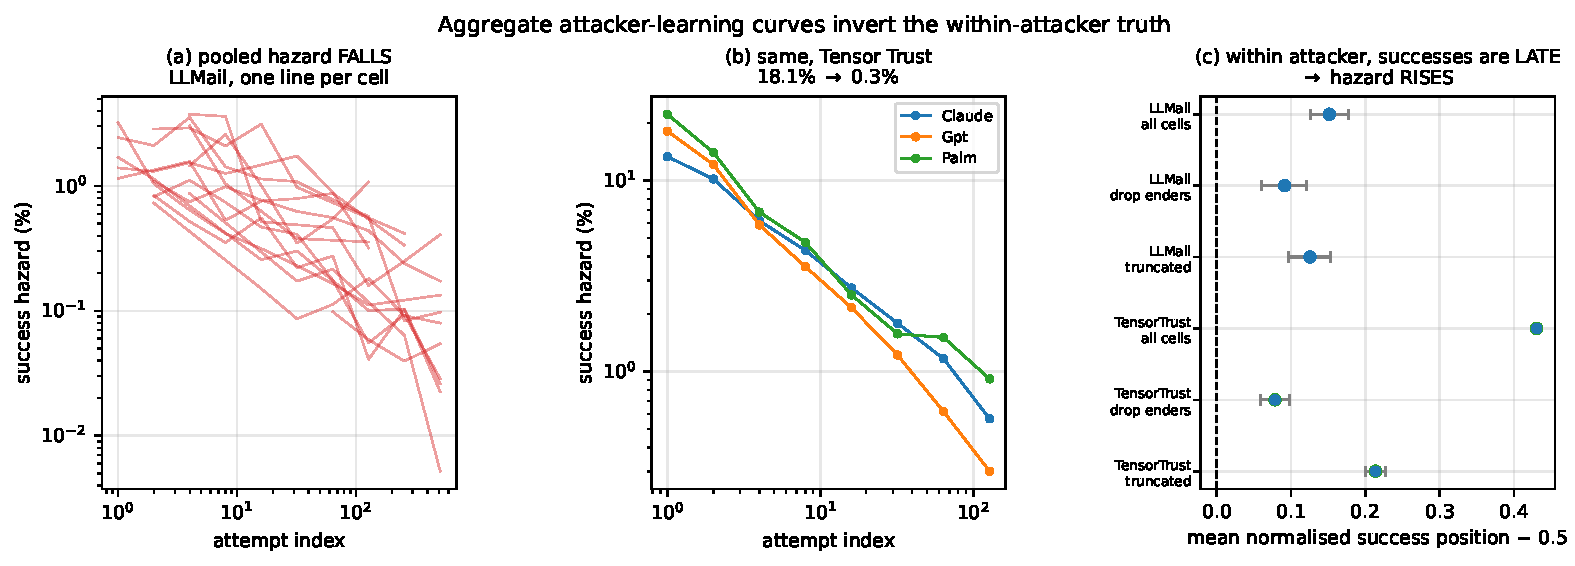
\includegraphics[width=\textwidth]{figs/F1_reversal.pdf}
\caption{(a) Pooled success hazard falls in every LLMail cell. (b) Tensor Trust: 18.1\% to 0.3\%, monotone, all three target models. (c) Conditioning on each attacker's own sequence, successes sit late under every stopping-rule treatment: the within-attacker hazard rises.}
\label{fig:F1_reversal}
\end{figure*}


A reader who takes this at face value concludes that attempts after the first few are nearly worthless, and that failure carries no exploitable information.


\subsection{Why the pooled curve cannot be trusted}

Let attacker \textit{i} have per-attempt success probability $h_{i}(n)$. The pooled hazard is

\begin{equation*}
h_{\mathrm{pop}}(n) \;=\; E\!\left[\, h_i(n) \;\middle|\; i \text{ has not succeeded before } n \,\right].
\end{equation*}

If attackers are heterogeneous in baseline hazard, meaning some are simply better, then those with high $h_{i}$ succeed early and leave the conditioning set, and the survivors at large \textit{n} are increasingly the low-$h_{i}$ ones. $h_{\mathrm{pop}}$ declines even if every $h_{i}$ is constant, and can decline even if every $h_{i}$ is rising. This is the frailty effect \cite{vaupel}, and it means the pooled curve is uninformative about individual learning without an explicit heterogeneity model.

Rather than model heterogeneity, we remove it.


\subsection{A frailty-proof estimator}

Condition on each cell's own attempt count \textit{N} and success count \textit{s}. Under the null of no within-attacker time structure, the \textit{s} success positions are a uniform random size-\textit{s} subset of \{1,\ldots,\textit{N}\}, whose mean normalized position is 0.5 regardless of \textit{N}, \textit{s}, or the attacker's skill. The statistic

\begin{equation*}
T \;=\; \operatorname{mean}(\text{success positions}) \,/\, N \;-\; 0.5
\end{equation*}

is therefore exactly zero in expectation under the null, for every attacker, and its sign gives the direction of the within-attacker trend: negative if successes cluster early (hazard declining), positive if late (hazard rising). Between-attacker heterogeneity cannot move it, because it is computed one attacker at a time against that attacker's own null.

\textbf{Censoring and informative stopping.} Write the observed sequence for cell \textit{c} as $Y_{c}$ = ($y_{\mathrm{1}}$,\ldots,$y_{\mathrm{N}}$\_c\}) with $y_{n}$ $\in$ \{0,1\}, and let $N_{c}$ be determined by a stopping rule \textit{$\tau_{c}$} that may depend on the history: attackers quit when satisfied, which in practice means shortly after a success. The stopping time is therefore \textit{informative}, in that $N_{c}$ is not independent of $Y_{c}$, and any statistic evaluated on the whole sequence inherits that dependence. Standard right-censoring machinery does not apply, because the censoring is triggered by the event.

Our truncation restores an ancillary window. Let $L_{c}$ = max\{\textit{n} : $y_{n}$ = 1\} be the last success and take the window $W_{c}$ = $L_{c}$ $-$ 1. Conditional on $L_{c}$, the stopping rule governs only what happens at and after $L_{c}$, so the sub-sequence ($y_{\mathrm{1}}$,\ldots,$y_{\mathrm{W}}$\_c\}) is free of it, and conditioning further on $s_{c}$ = $\Sigma$\_\{n$\le$$\_{c}$ $y_{n}$ makes the success positions exchangeable under the null. Both the position statistic \textit{T} and the conditional likelihood of \S4.5 are computed on this window, so neither depends on the stopping rule. The cost is that cells with a single success contribute nothing (their window contains no events) and cells that never succeed contribute nothing under any within-cell design (\S4.5). We therefore report the untruncated estimator alongside as an explicit bound: it is biased \textit{toward} our conclusion, and we never rely on it.

One complication remains: attackers tend to stop once they succeed, which by construction places the final success at position \textit{N} and biases \textit{T} upward. We handle this three ways (Table 1). Estimator A ignores it, which is conservative against the hypothesis we are about to reject but biased toward the one we accept. Estimator B drops cells whose last attempt is a success. Estimator T truncates each cell to attempts before its last success and evaluates the remaining successes in that window, which the stopping rule cannot touch. T is primary.

\begin{table*}[t]
\centering
\caption{Within-attacker success position, mean(\textit{T}) with 95\% bootstrap CI over cells.}
\label{tab:1}
\small
\begin{tabular}{lcc}
\toprule
\textsc{estimator} & \textsc{LLMail} & \textsc{Tensor Trust} \\
\midrule
A --- all cells & +0.152 [+0.127, +0.177] (377) & +0.430 [+0.427, +0.433] (9,273) \\
B --- drop cells ending in success & +0.091 [+0.061, +0.121] (267) & +0.078 [+0.059, +0.098] (731) \\
\textbf{T --- truncated window} & \textbf{+0.125 [+0.097, +0.154] (291)} & \textbf{+0.214 [+0.201, +0.227] (1,469)} \\
\bottomrule
\end{tabular}
\end{table*}


All six estimates are positive and exclude zero, and no cell or arm in either corpus came out negative. Within an attacker, successes come late, so the hazard rises (Figure 1(c)).


\subsection{Independent confirmation and a permutation null}

Estimator \textit{T} is position-based. To rule out an artefact of that construction we use a second estimator sharing none of its form: inside each truncated window, compare the empirical success \textit{rate} in the second half of attempts to the first. We test it against a within-cell label permutation null, which shuffles each attacker's own success labels across their own attempts. This destroys within-attacker time structure while preserving \textit{N}, \textit{s}, and every between-attacker difference exactly.

\begin{table*}[t]
\centering
\caption{Split-half rate difference, second half minus first, with permutation null (2,000 permutations).}
\label{tab:2}
\small
\begin{tabular}{lccccc}
\toprule
\textsc{corpus} & \textsc{windows} & \textsc{rate difference} & \textsc{95\% CI} & \textsc{null mean (sd)} & \textsc{one-sided }\textit{p} \\
\midrule
LLMail & 286 & +0.0265 & [+0.0133, +0.0407] & +0.0002 (0.005) & \textless{} 0.001 \\
Tensor Trust & 1,129 & +0.1020 & [+0.0873, +0.1171] & +0.0004 (0.007) & \textless{} 0.001 \\
\bottomrule
\end{tabular}
\end{table*}


The observed statistic sits 5--15 standard deviations outside a null that preserves frailty exactly. No permutation of 2,000 reached the observed value in either corpus, so the one-sided \textit{p} is at the resolution floor of 1/(\textit{B}+1) and we report it as an upper bound rather than a point estimate. Frailty alone cannot produce this.


\subsection{Effect size: conditional logistic regression with attacker fixed effects}

To put a number on the trend we fit, within each cell,

\begin{equation*}
\operatorname{logit} \Pr\!\left[\text{success at attempt } n\right] \;=\; \alpha_c + \beta \log n,
\end{equation*}

and condition on each cell's own success count, which eliminates $\alpha_{c}$, and with it attacker skill, exactly. The conditional likelihood sums over all size-\textit{s} subsets of the window; we evaluate it by the standard clogit dynamic programme in log space, which is exact for every cell including LLMail windows holding 554 successes. Confidence intervals are profile-likelihood. The implementation was checked against brute-force enumeration over all subsets and recovers known $\beta$ on simulated data with heterogeneous $\alpha$.

\begin{table*}[t]
\centering
\caption{Conditional logistic regression with attacker fixed effects.}
\label{tab:3}
\small
\begin{tabular}{lccc}
\toprule
\textsc{corpus} & \textsc{windows} & \textsc{$\beta$} & \textsc{hazard ratio per doubling of attempt index} \\
\midrule
LLMail & 291 & +0.056 [+0.017, +0.097] & 1.040$\times$ [1.012, 1.069] \\
Tensor Trust & 1,449 & +1.077 [+0.999, +1.156] & 2.109$\times$ [1.998, 2.228] \\
\bottomrule
\end{tabular}
\end{table*}


Going from attempt \textit{n} to attempt 2\textit{n} multiplies a Tensor Trust attacker's per-attempt success probability by 2.11, and an LLMail attacker's by 1.04. Both intervals exclude 1. The LLMail effect is small in magnitude, though its interval excludes 1. The nonparametric results of \S4.3 and \S4.4 remain the primary evidence for the sign; this section supplies the scale.

Two properties of the estimand deserve statement. First, cells with zero successes (71.8\% of LLMail cells and 55.5\% of Tensor Trust cells) contribute a likelihood that is constant in $\beta$, and are therefore uninformative about a within-cell trend. This is not a filtering choice: \textit{no} fixed-effects design can use them, because a cell with no outcome variation carries no within-cell information. The estimator is silent about attackers who never break through, and our claims are correspondingly about attackers who do. Second, fitting the same model on full sequences rather than truncated windows drives $\beta$ to the optimizer boundary on Tensor Trust ($\beta$ = 3.000). That is a direct measure of how severe the stopping-rule bias is, and of why the truncated window is primary. On simulation the estimator carries a mild upward bias in \textbar{}$\beta$\textbar{} at large effect sizes under the 0 \textless{} \textit{s} \textless{} \textit{W} conditioning (recovering 0.84 for a true 0.80), so magnitudes should be read as approximate; signs and intervals are unaffected.


\subsection{Ruling out alternatives}

\textit{Community diffusion.} Within an attacker, attempt index and wall-clock time are collinear; a technique spreading publicly mid-challenge would look like individual learning. Restricting to attackers whose entire sequence falls inside a single sitting removes the time for diffusion. At a span of 6 hours or less, Tensor Trust attackers show +0.107 [+0.026, +0.188] (44 windows), the same magnitude as the unrestricted +0.102; at 24 hours or less the estimate is +0.089 [+0.034, +0.143] (92 windows). LLMail at $\le$ 24 hours: +0.075 [+0.010, +0.148] (43). There is no dose-response with span, which diffusion would produce. Attackers who finish inside a single sitting are of course a self-selected subgroup, so this test bounds the diffusion explanation rather than eliminating every temporal confound.

We note for anyone reproducing this that a \textit{between}-attacker version of the calendar test, comparing high- to low-attempt-index attempts within a calendar bin across attackers, reports the effect reversing. That test is invalid: attackers sitting at high attempt index at any moment are those who have been grinding without success, so it re-measures frailty. It is exactly the error this section corrects.

\textit{Level progression.} LLMail cells pool difficulty levels 1--4, and teams progress to harder levels over time, which should bias against learning. Holding level fixed, the split-half effect is stronger, not weaker: +0.042 [+0.024, +0.061] over 238 windows.

\textit{Clustering.} Successes cluster (\S5), and one might worry the permutation test conflates clustering with trend. The single-success-window fit of \S4.5, in which no clustering is possible, is positive on both corpora.


\section{Attackers Learn from Success, by Mutation}

The rising hazard of \S4 says attackers extract information from failure. They extract far more from success.

\textbf{The second success comes faster.} Among cells with at least two successes, we compare the gap from the first success to the second against the gap to the first. In Tensor Trust the second gap is shorter for 46--62\% of attackers, against a per-cell constant-hazard null of 24--29\%, with \textit{p} \textless{} 0.001 in each of the three target-model arms. In LLMail the same statistic is 64.7\% pooled over 286 teams in 15 cells, against that corpus's own constant-hazard null of approximately 48\%; the per-cell values range from 20\% to 100\%, and two of the fifteen cells fall below 50\%. Tested individually against their own nulls, 2 of 8 phase-1 LLMail cells reach significance (both Prompt Shield arms, \textit{p} \textless{} 0.001), three are marginal at \textit{p} $\approx$ 0.07, and three are not significant, which we attribute to per-cell samples of 11 to 72 teams. The direction is consistent across cells; the LLMail evidence for this claim is weaker than the Tensor Trust evidence, and the replication rests on the latter.

\textbf{It is a variant, not a rediscovery.} In LLMail phase 2 (the phase with payload text), the second successful payload has median Jaccard similarity 0.89 to the first, but only 14\% are exact copies. Attackers take the payload that worked and mutate it. Team 2's own write-up in the LLMail appendix describes the process: an LLM was used ``to repeatedly generate new email bodies that matched the working email structure but different in wording'', yielding ``one successful bypass for every 10--15 email variants''.

\textbf{Knowledge does not transfer across defenses.} For the 29 teams that attacked two defenses, the gap to first success on the second defense is shorter than on the first only 48\% of the time, which is chance. What transfers is the exploit rather than a general skill.

\textbf{Family construction.} Within a cell we take the first end-to-end success as the family seed and admit every \textit{subsequently submitted} payload within the similarity threshold of that seed; membership is defined against the seed, not transitively, so a family cannot drift arbitrarily far from its origin by chains of small edits. Because families are seeded per cell, one attacker attacking two defenses produces two independent families, and a payload text submitted by two different attackers belongs to both of theirs. For the judge experiment of \S7 we de-duplicate at the level of payload text before inference, collapsing 18,315 (family, payload) pairs to 9,392 distinct strings, then re-expand afterwards, so a string shared across families is scored once and counted in each. Exact resubmissions of the seed are tracked separately from near-variants throughout and never counted as family members.

A working payload is thus the seed of an \textit{exploit family}, and after the first success an attacker's throughput is governed by how much of that family the defense lets through.


\section{Family Survival Rate}


\subsection{Definition}

Let \textit{P} be a payload that evaded defense \textit{D}, and let \textit{V}(\textit{P}) be the set of subsequently submitted payloads within Jaccard token similarity 0.7 of \textit{P}. The \textbf{family survival rate} of \textit{D} is

\begin{equation*}
\mathrm{FSR}(D) \;=\; \Pr\!\left[\, v \text{ evades } D \;\middle|\; v \in V(P),\; P \text{ evaded } D \,\right],
\end{equation*}

estimated over all families and reported with a family-level bootstrap.

\textbf{Two admissible seed definitions.} ``\textit{P} evaded \textit{D}'' can mean \textit{P} got past the detector, or that \textit{P} achieved end-to-end success (retrieved, evaded, and fired the tool with correct arguments). The first is the narrower statement about \textit{D}; the second is what the attacker was actually trying to do. Both are defensible and they give materially different numbers, so we report the sensitivity rather than choosing silently. The pooled table below uses the detector seed, matching the definition above; the paired analysis of \S6.3 uses the end-to-end seed, which is the more conservative of the two for our claim. FSR measures local robustness in the neighbourhood of a defense's own failures, under the mutation distribution the attackers happened to use; it is therefore a property of the defense--mutation-distribution pair, not of the defense in isolation. ASR cannot see it: ASR treats attempts as exchangeable, and FSR is a statement about their dependence.

\textbf{FSR is a property of a (defense, mutation-distribution) pair.} The neighbourhood \textit{V}(\textit{P}) is populated by whatever variants the attackers actually submitted, so FSR confounds the defense's local behaviour with how those particular attackers mutate. This matters differently in our two corpora. Tensor Trust is uncrossed, in that each defense faces a different, self-selected set of attackers. Its cross-defense spread (\S6.2) therefore mixes defense effects with attacker mix, and we report it as evidence that FSR varies widely in the wild rather than as a ranking of defenses. LLMail is crossed, and the paired design of \S6.3 holds the attacker constant on both sides of every comparison; that is where the claim about defenses rests. Any FSR reported against an automated attacker measures the pair (defense, search operator) and should be read accordingly (\S2).


\subsection{FSR varies by an order of magnitude}

On LLMail, with the detector-level evasion flag and target model held fixed (Figure 2b):


\begin{figure}[t]
\centering
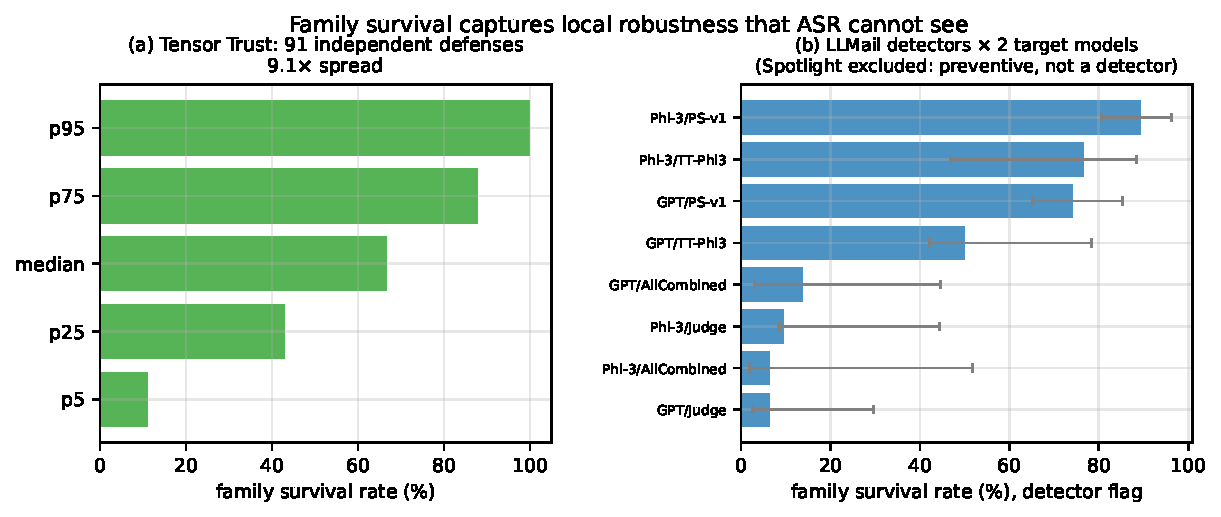
\includegraphics[width=\columnwidth]{figs/F2_fsr_variation.pdf}
\caption{Family survival rate, which measures local robustness under an observed attacker mutation distribution. (a) 91 Tensor Trust defenses span 11\% to 100\%. (b) LLMail detectors on both target models; Spotlight is excluded because it is preventive and the detector flag is true for it by construction.}
\label{fig:F2_fsr_variation}
\end{figure}


\begin{table}[t]
\centering
\caption{Family survival rate on LLMail, detector-level evasion flag.}
\label{tab:4}
\small
\begin{tabular}{lcc}
\toprule
\textsc{defense} & \textsc{Phi-3} & \textsc{GPT-4o-mini} \\
\midrule
Prompt Shield & 89\% [81, 96] & 74\% [65, 85] \\
TaskTracker & 77\% [47, 88] & 50\% [42, 78] \\
LLM judge & 10\% [8, 44] & 6\% [3, 30] \\
\bottomrule
\end{tabular}
\end{table}


Under the end-to-end seed the same pooled quantities are 36.6\% / 50.1\% (LLM judge, GPT / Phi-3), 38.1\% / 88.5\% (Prompt Shield), and 43.8\% / 84.4\% (TaskTracker). The judge remains lowest on both target models under both definitions, but its margin over Prompt Shield on GPT is large under one seed (6.3\% vs 74.2\%) and slight under the other (36.6\% vs 38.1\%). We therefore do not claim a magnitude for the pooled comparison; \S6.3 is where the defense claim is tested.

On Tensor Trust, across 91 independent defenses with at least ten near-variants (Figure 2a), the 5th percentile is 11.0\%, the median 66.7\% and the 95th percentile 100.0\%, a 9.1$\times$ spread. This is not an artefact of four hand-built defenses.

The ten-variant cutoff is a precision floor, and it selects heavily: of 906 defenses with at least one near-variant, it retains 91 (10.0\%). The direction of that selection runs against the claim rather than for it: the 815 excluded defenses have a mean FSR of 92.2\%, against 62.4\% for those retained. The reported distribution is therefore conservative with respect to the claim that family survival is often high. (The excluded estimates are individually near-worthless, being computed on one to nine variants and piling up at 0 and 1; the comparison establishes direction, not magnitude.) The spread itself is not an artefact of the cutoff: it is 9.3$\times$ at a cutoff of 20 defenses and 6.1$\times$ at 50.

\textbf{How much of this is the defense, and how much the attacker?} Because Tensor Trust is uncrossed we can bound the answer by comparing dispersions. Per-defense FSR (n $\ge$ 10) has standard deviation 0.292 across 91 defenses; per-\textit{attacker} FSR, computed identically, has standard deviation 0.269 across 56 attackers. Attacker identity accounts for very nearly as much variation as defense identity. We therefore do not read \S6.2 as a ranking of defenses. It establishes that family survival varies widely in deployed conditions, which is the claim that matters for evaluation practice. The defense-level claim rests entirely on the paired design below.


\subsection{It survives a paired design}

Teams chose which LLMail defenses to attack, so cross-defense comparisons are confounded by who attacked what. Restricting to teams that attacked \textit{both} members of a pair, and computing each team's FSR on each, gives a paired comparison in which the attacker is their own control (Figure 3). Seven of twelve defense pairs differ significantly. The LLM judge has lower FSR than Prompt Shield on both target models: $-$32.4 points [$-$49.3, $-$16.4] on GPT-4o-mini and $-$6.7 [$-$13.1, $-$2.0] on Phi-3.


\begin{figure}[t]
\centering
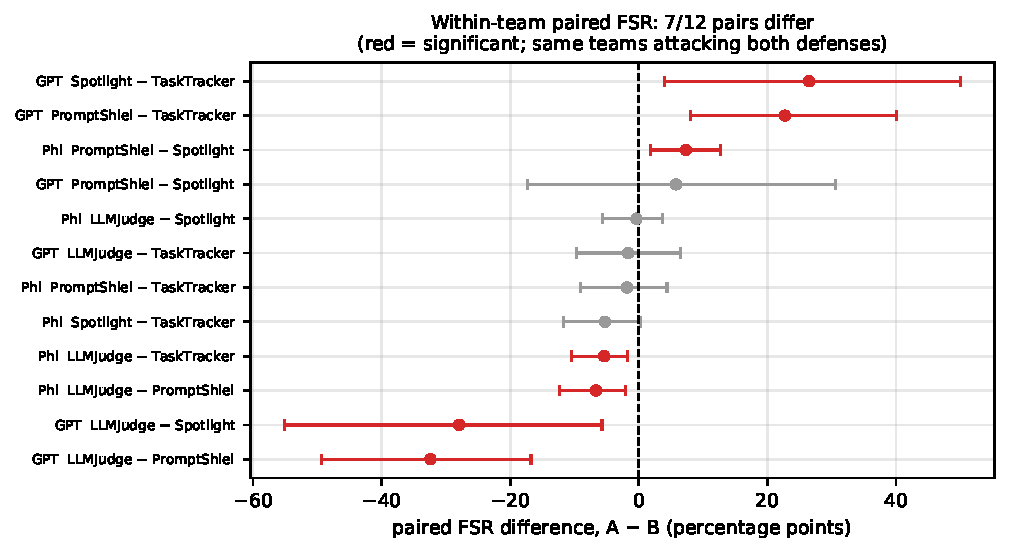
\includegraphics[width=\columnwidth]{figs/F3_paired_fsr.pdf}
\caption{Within-team paired FSR on LLMail: the same teams attacking both defenses of a pair. Seven of twelve pairs differ; intervals excluding zero are marked.}
\label{fig:F3_paired_fsr}
\end{figure}


This is the one comparison we rely on, so we repeat it under the alternative seed definition. With the detector seed, the same paired contrast gives $-$53.4 points [$-$71.5, $-$32.9] on GPT and $-$42.9 [$-$65.6, $-$20.0] on Phi-3, and 15 of 17 pairs differ (the larger pair count reflects Spotlight becoming comparable under that flag, though its detector-level FSR is 100\% by construction and we exclude it from ranking claims). Judge-below-Prompt-Shield is thus significant in all four combinations of target model and seed definition, with the point estimate ranging from $-$6.7 to $-$53.4 points. Sign and significance are robust; magnitude is not, and we claim only the former.


\subsection{What is and is not robust}

Token-set Jaccard is order-blind, and a reader may reasonably worry it admits structural rewrites alongside superficial rewords. Recomputing FSR under a character 5-gram measure and an order-sensitive sequence-ratio measure over token sequences, at thresholds 0.7 and 0.85, the LLM judge and the all-defenses arm remain the two lowest under every measure. Absolute values shift by a few points; the ordering claim does not.

The claim that the LLM judge has the lowest family survival holds on both target models, in the paired design, and at every near-variant threshold from Jaccard 0.5 to 0.9. The \textit{full ordering} among the remaining defenses does not: Prompt Shield versus TaskTracker reverses between target models and shifts with the threshold. We therefore claim only the former.


\section{A Negative Result: Determinism Does Not Explain FSR}

The natural hypothesis is that FSR is governed by decision-boundary determinism. A deterministic classifier that passes \textit{P} should pass small perturbations of \textit{P}; a stochastic judge, sampling its verdict, has no stable neighbourhood to exploit. Two LLMail measurements are consistent with this: on exact resubmission of a payload that passed, Prompt Shield passes it again 99.7\% of the time and TaskTracker 96\%, while the LLM judge passes it only 51--71\% of the time, and the judge has the lowest FSR.

The hypothesis fails two tests.

\textbf{It does not replicate.} Tensor Trust defenses are near-deterministic, passing 89--96\% of exact resubmissions across all three target models, yet their pooled FSR is only about 30\%. Determinism is therefore at most necessary, and not sufficient.

\textbf{It fails a causal test, and the failure is directional.} We replayed the 242 real LLMail exploit families (16,469 near-variants) through an open-weights judge (Qwen2.5-1.5B-Instruct) at four temperatures, holding the family set, scoring rule and threshold identical across arms. Sampling was verified to be real and graded: decision consistency across draws falls monotonically with temperature.

\begin{table*}[t]
\centering
\caption{Temperature dose-response. Consistency is the probability that two draws agree on the same payload; FSR is measured over the same 242 families in every arm.}
\label{tab:5}
\small
\begin{tabular}{lccc}
\toprule
\textsc{temperature} & \textsc{consistency} & \textsc{FSR} & \textsc{95\% CI} \\
\midrule
0.0 & 0.996 & 8.65\% & [4.6, 14.7] \\
0.3 & 0.934 & 8.73\% & [4.7, 14.8] \\
0.7 & 0.824 & 11.04\% & [6.4, 18.0] \\
1.0 & 0.725 & 13.64\% & [9.2, 19.4] \\
\bottomrule
\end{tabular}
\end{table*}


Every pairwise contrast between arms has overlapping intervals, but pairwise testing is the wrong instrument for an ordered dose-response: it discards the ordering and pays a multiplicity cost for nothing. Regressing FSR on temperature and bootstrapping over families gives a slope of \textbf{+5.10 FSR points per unit temperature, 95\% CI [+3.15, +6.67], with P(slope $\le$ 0) \textless{} 0.001}. The mechanism predicts a \textit{negative} slope. This is evidence \textit{against} it, not merely absence of evidence for it.

Nor is it an artefact of one judge size. Repeating the two-temperature contrast with Qwen2.5-7B-Instruct gives FSR 10.73\% [4.7, 20.2] at temperature 0 and 11.43\% [5.3, 21.1] at temperature 1.0, the same direction, with consistency falling from 0.997 to 0.903. Both judges come from one model family and share a single prompt, so the result is established for these judges and this prompt; we do not claim it for guardrails built differently.

A plausible reading is that two effects compete. Randomizing the boundary removes the neighbourhood structure a found exploit sits in, which helps the defender, but it also gives the attacker an independent re-roll on every variant, including ones a deterministic judge would always have caught. In the judge configurations tested here the second effect dominates: each increment of randomization buys the attacker more in re-rolls than it costs in lost structure. We therefore find no support for randomizing a detector's decision boundary as a way to suppress exploit families, and in these configurations it moved family survival in the opposite direction. Whether that holds for guardrails built differently is untested.

\textbf{A pitfall worth recording.} Our first run of this experiment scored the judge by the ratio Pr[YES] / (Pr[YES] + Pr[NO]) from first-token log-probabilities and thresholded at 0.5. That quantity is exactly temperature-invariant, because temperature scaling raises both logits to the power 1/\textit{T}, which cannot change which is larger. The ``sampled'' arm was therefore not sampled (consistency 0.990 against 0.995) and returned an uninformative null. Scoring from the judge's actually emitted verdict is required. We expect this mistake to be common.


\section{Discussion}

\textbf{For evaluation.} Any statistic of the form ``attackers succeed within \textit{k} attempts'' or ``success rate at attempt \textit{n}'', computed by pooling over attackers, inherits the frailty confound and will understate individual learning, potentially to the point of reversing its sign, as here. The frailty-proof estimators of \S4 cost nothing beyond attacker identifiers, which both public corpora already provide. We recommend that adaptive-attack evaluations report within-attacker statistics or not report learning curves at all.

\textbf{For defense design.} ASR answers ``what fraction of independent attempts get through''. Against an adaptive attacker who mutates successes, the operative question is ``once one gets through, how many of its neighbours do'', and that is FSR. Two defenses with the same ASR can differ tenfold in FSR. Because FSR is measured against a particular mutation distribution, it characterises a defense only relative to the attacker population that produced the variants. The LLM judge in LLMail has both the lowest ASR and the lowest FSR, so the two agree there; but the paired analysis shows they disagree among the other defenses, and on Tensor Trust FSR spans nearly the whole unit interval. We suggest FSR be reported alongside ASR whenever adaptive-attack data are available.

\textbf{For the mechanism.} We do not know what governs FSR. Determinism is not merely insufficient: in the configurations of \S7 the dose-response runs significantly in the opposite direction, so randomizing a detector's boundary is not a reliable way to suppress exploit families. A descriptive correlation between FSR and the similarity of surviving variants (\textit{r} = +0.52 over eight defense-cells) hints that FSR may track how well a defense's decision boundary aligns with the attacker's mutation space, with trained surface classifiers aligned to token-level edits and generative decisions less so. Eight points are not evidence, and we leave this open.


\section{Limitations}

Both corpora are challenge or game data; participants may behave differently from adversaries with real incentives, and LLMail's five-flag feedback is richer than a silent production deployment provides. Our near-variant threshold is a token-set Jaccard at 0.7; the ``judge lowest'' claim is robust from 0.5 to 0.9, under order-sensitive and character-n-gram similarity, and under both family-seed definitions, while the finer ordering and all magnitudes are not. FSR values depend materially on whether a family is seeded by detector evasion or by end-to-end success (the judge's pooled FSR on GPT is 6.3\% under one and 36.6\% under the other), which is why we claim only the sign of the paired contrast. FSR is defined against the mutation distribution the attackers happened to use, so the Tensor Trust spread partly reflects attacker mix; only the LLMail paired comparisons hold the attacker fixed. The ten-near-variant cutoff on Tensor Trust selects defenses that attackers persisted against; we report the retained fraction and the excluded defenses' FSR rather than assuming the selection is benign. Within-cell fixed-effects estimation is structurally silent about attackers who never succeed (71.8\% of LLMail cells, 55.5\% of Tensor Trust), so the learning claim is about attackers who eventually break through. The LLMail hazard ratio is small (1.04$\times$ per doubling) though its interval excludes 1, and the conditional-likelihood estimator shows mild upward bias in \textbar{}$\beta$\textbar{} at large effect sizes on simulation. The causal experiment covers two judges (1.5B and 7B) and four temperatures, but one prompt and one model family; whether the positive slope holds for a differently-constructed guardrail is untested. Its calibration set is 160 unique benign emails. The threshold question dissolves under sampled-label scoring: the judge emits a verdict rather than a score, so values are binary and every threshold in (0,1) induces the same partition; the 0.5-floor and strict FPR-matched analyses return identical numbers. vLLM inference at temperature 0 is not bit-reproducible under shuffled batching (3.2\% of scores identical) though decisions agree 99.5\%; we report the ``deterministic'' arm as near-deterministic. Finally, one methodological pitfall is documented in \S7 because it is reproducible and easy to repeat: scoring an LLM judge by a normalised two-way log-probability ratio and thresholding it is temperature-invariant, so an experiment varying temperature under that scoring rule cannot detect an effect of temperature and will return an uninformative null.


\section{Conclusion}

The learning curve the field has been reading is a survivorship curve. Corrected for heterogeneity, human attackers against LLM defenses learn from failure within a target and learn from success across targets by mutating what worked into a family of exploits. The first fact means adaptive-attack evaluations built on pooled statistics understate the threat. The second means that attack success rate, which treats attempts as independent, cannot see the mechanism by which one success becomes many. We offer family survival rate, measured against an observed attacker mutation distribution, as a metric that can.


\section{Open Science}

The artifact accompanying this paper contains the analysis code, the preprocessing scripts that build the derived corpora from the public raw dumps, the result files backing every table and figure, the raw per-payload judge outputs behind \S7, the figure-generation scripts, a dependency specification, and a verification harness.

Both datasets are public and are not redistributed here. LLMail-Inject is available from the Hugging Face dataset \texttt{microsoft/llmail-inject-challenge} under the MIT licence \cite{llmail}; Tensor Trust is available from the authors' repository \cite{tensortrust}. The artifact's README gives the download commands and the preprocessing steps that turn the raw dumps into the derived files the analyses read.

\texttt{python verify.py} checks every headline quantity in this paper and reports PASS or FAIL per quantity. \texttt{python verify.py --rerun} additionally re-executes the CPU analysis pipeline from the derived corpora before verifying, so a reviewer can confirm that the numbers reported here are the numbers the code produces. Producing the \S7 judge decisions in the first place requires a GPU, but the raw per-payload outputs of all six arms are included in the artifact, together with the payload-to-family index they are analysed against. Every \S7 quantity reported here, including the per-arm decision consistency, the family survival rates and their intervals, the temperature slope and the second-judge replication, is recomputed from those raw outputs each time \texttt{verify.py} runs rather than read back from a stored summary, so \S7 can be checked without a GPU.


\section{LLM Usage Considerations}

\textit{LLMs as objects of study.} The experiments in \S7 use Qwen2.5-1.5B-Instruct and Qwen2.5-7B-Instruct as injection-detection judges, served locally with vLLM. The corpora analysed throughout were produced by human attackers against LLM-based systems: LLMail-Inject targets Phi-3-medium-128k-instruct and GPT-4o-mini, and Tensor Trust targets GPT-3.5-turbo, Claude Instant 1.2 and PaLM chat-bison. These models are experimental subjects, not tools of the analysis.

\textit{Editorial use.} LLMs were used for editorial purposes in this manuscript, and all outputs were inspected by the author to ensure accuracy and originality.

\textit{LLM assistance in conducting the research.} An AI coding assistant was used substantially throughout this work: writing and debugging the analysis and preprocessing code, implementing the statistical estimators, searching and screening related literature, drafting and editing the manuscript, organising the repository, and preparing the artifact. Several analytical errors were introduced and subsequently caught during that process, including the temperature-invariant scoring rule documented in \S7.

\textit{Originality and responsibility.} The author is solely responsible for the entire content of this paper, including all text and figures. That responsibility includes verifying the analysis code, the experimental outputs, the statistical procedures and their interpretation, the bibliography, and the final manuscript; it is not diminished by the use of AI assistance in producing any of them. Every bibliographic entry was checked against a primary source, and every quantitative claim is reproduced by the accompanying verification harness.

\textit{Limitations of the assistance and how they were handled.} AI assistance introduced errors that survived until they were caught by explicit testing rather than by inspection. Two are documented in this paper because they are instructive: the temperature-invariant scoring rule of \S7, which produced a plausible but meaningless null; and a bibliographic entry whose author list was fabricated and was corrected only after verification against Crossref and DBLP. The mitigations adopted were to require that every reported quantity be regenerated by a scripted pipeline rather than transcribed, that estimators be validated against synthetic data with known ground truth before being applied, and that every reference be confirmed against a primary source. Readers should weigh the possibility that further errors remain.

\textit{Model and compute choices.} The \S7 judges are Qwen2.5-1.5B-Instruct and Qwen2.5-7B-Instruct. Open-weight models served locally were necessary rather than convenient: the experiment manipulates sampling temperature and measures decision consistency, which requires control over the decoding path and a reproducible greedy mode. Hosted APIs do not guarantee deterministic decoding, so an API judge could not have supported the temperature contrast. The 1.5B model was chosen after the 7B model proved unusable for this measurement: at a matched operating point it flagged essentially every payload, leaving no variation in which to observe family survival. The 7B model is retained as the second-judge replication, where a two-temperature contrast is still informative.

\textit{Computational footprint.} All \S7 runs together used approximately three GPU-hours on a single rented consumer GPU (NVIDIA RTX 4090), comprising roughly 300,000 judge inferences over 9,392 distinct payloads at four temperatures with repeated draws. No model was trained or fine-tuned; all use was inference with published open-weights checkpoints. Compute was limited by de-duplicating payloads before inference (18,315 pairs to 9,392 strings), by making runs resumable so no work was repeated after an interruption, and by running a 200-payload timing probe before committing to each full run. Every other analysis in this paper runs on a laptop CPU in minutes. The corpora were collected by prior work, so this study required no new data collection from human participants.

\bibliographystyle{IEEEtran}
\bibliography{refs}

\end{document}
